\documentclass[10pt, a4paper]{article}

\usepackage{ctex}
\usepackage{xeCJK}
\usepackage{caption}
\usepackage{geometry}
\geometry{
    left = 0.6in,
    right = 0.6in,
    top = 0.8in,
    bottom = 1.0in
}
\usepackage{amssymb}
\usepackage{amsbsy}
\usepackage{amsmath}
\usepackage{xcolor}
\usepackage{mathrsfs}
\usepackage{graphicx}
\usepackage{pifont}
\usepackage{tasks}
\settasks{
    label = \Alph*. ,
    label-width = 16pt
}
\pagestyle{empty}

\newcommand{\Title}[3]{
    \begin{center}
        \Large \textbf{中国电子学会 #1~年~#2~月 Scratch~#3级考试}
    \end{center}
}
\newcommand{\TimeAndName}[1]{
    \begin{center}
        考试时间:~#1~ 分钟 \qquad\qquad\qquad\qquad 姓名:\underline{\quad\quad\quad\quad}
    \end{center}
}

\begin{document}
    \Title{2022}{6}{二} % 标题
    \TimeAndName{60} % 考试时间及姓名

    % 单选题
    \vspace{2mm}
    {\noindent\textbf{第一部分、单选题(共 25 题,每题 2 分,共50分.)}}
    \begin{enumerate}
        % 1
        \item 角色初始位置在舞台正中间,下面哪个选项能让角色移到舞台的左下角?(\qquad)
        \begin{tasks}(4)
            \task 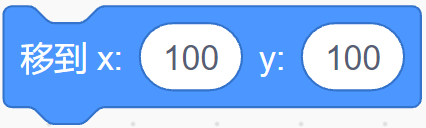
\includegraphics[width=.18\textwidth]{1a.png}
            \task 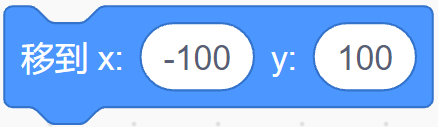
\includegraphics[width=.18\textwidth]{1b.png}
            \task 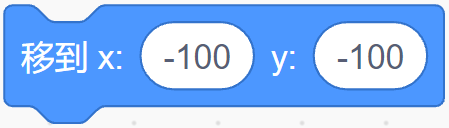
\includegraphics[width=.18\textwidth]{1c.png}
            \task 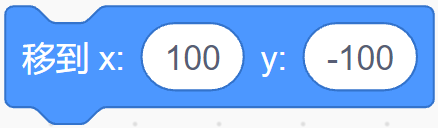
\includegraphics[width=.18\textwidth]{1d.png}
        \end{tasks}

        % 2
        \item 点击绿旗,执行下面程序,关于小鱼的运动描述正确的是?(\qquad)
        \begin{tasks}(2)
            \task 小鱼不会动
            \task 小鱼一会向上游,一会向下游
            \task 按下空格键小鱼向上游,松开空格键小鱼就不动
            \task 按下空格键小鱼往前游,松开空格键小鱼就往后退
        \end{tasks}

        % 2,3,6 图片
        \begin{figure}[htbp]
            \begin{minipage}[t]{.35\textwidth}
                \centering
                \begin{minipage}[t]{.45\textwidth}
                    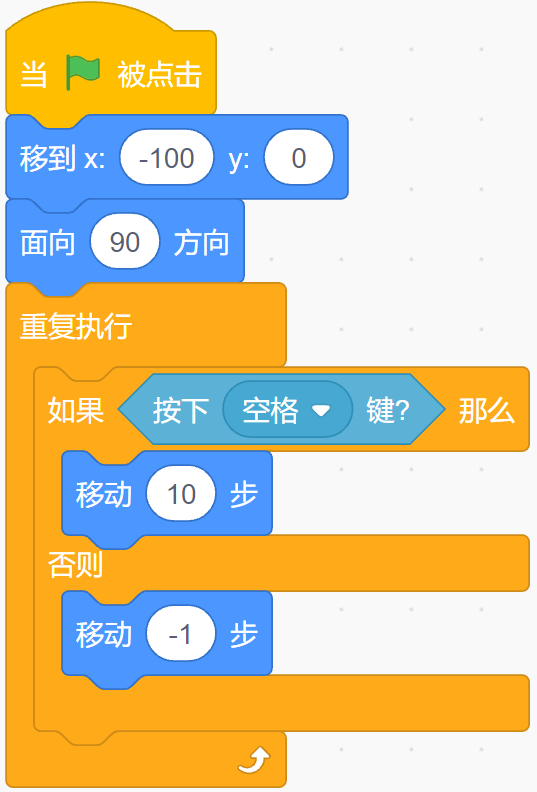
\includegraphics[width=\textwidth]{2-1.png}
                \end{minipage}
                \begin{minipage}[t]{.53\textwidth}
                    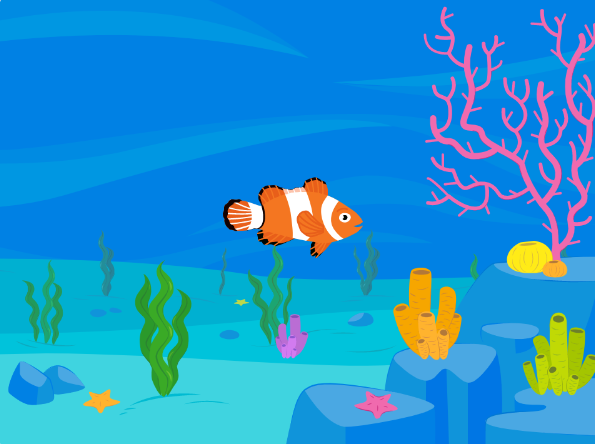
\includegraphics[width=\textwidth]{2-2.png}
                \end{minipage}
                \caption*{第 2 题}
            \end{minipage}
            \begin{minipage}[t]{.25\textwidth}
                \centering
                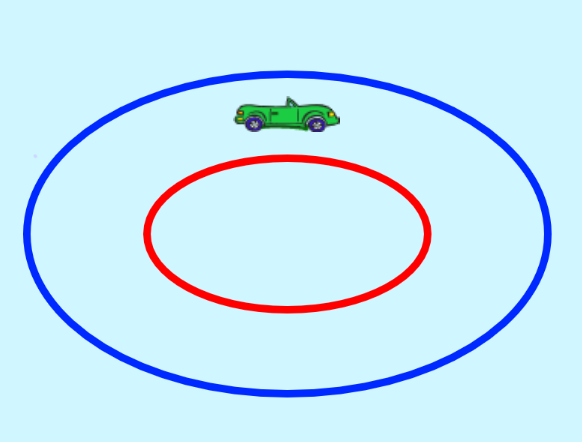
\includegraphics[width=\textwidth]{3.png}
                \caption*{第 3 题}
            \end{minipage}
            \begin{minipage}[t]{.35\textwidth}
                \centering
                \begin{minipage}[t]{.45\textwidth}
                    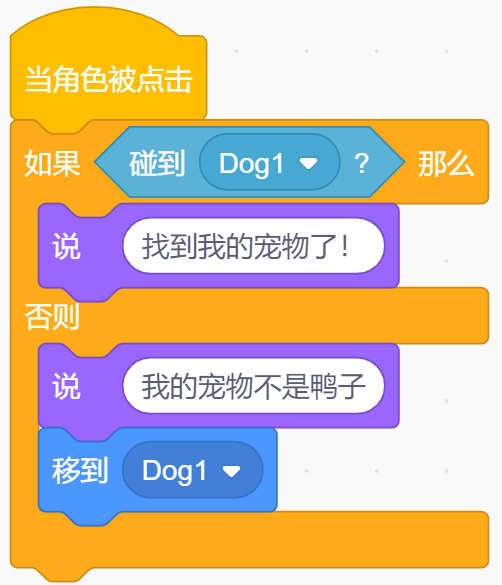
\includegraphics[width=\textwidth]{5-1.png}
                \end{minipage}
                \begin{minipage}[t]{.53\textwidth}
                    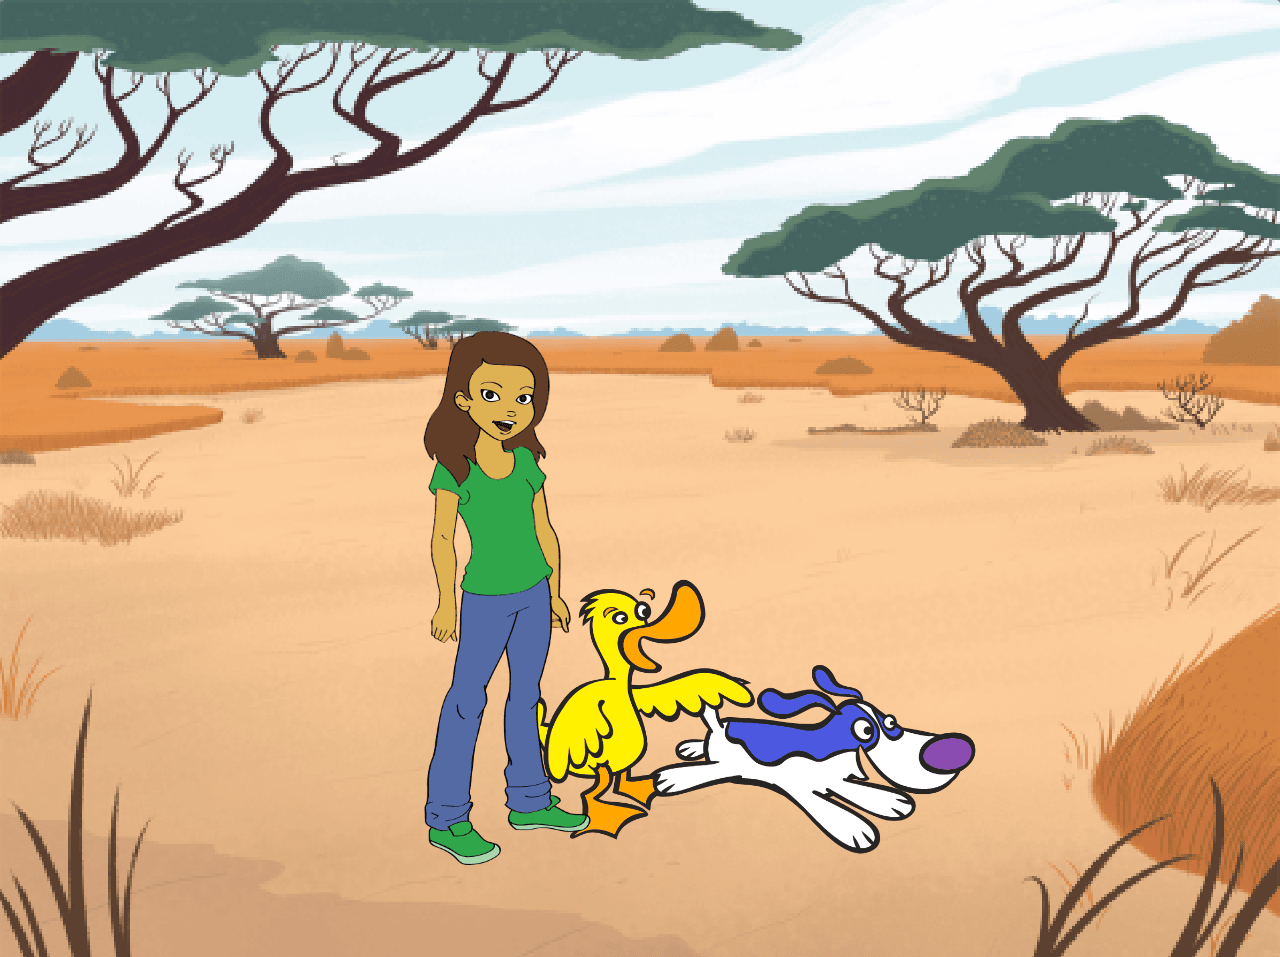
\includegraphics[width=\textwidth]{5-2.png}
                \end{minipage}
                \caption*{第 5 题}
            \end{minipage}
        \end{figure}

        % 3
        \item 做一个赛车游戏,车的初始方向面向右,车的左边是蓝色赛道,右边是红色赛道,以下哪个选项能实现赛车始终在赛道内前进?(\qquad)
        \begin{tasks}(4)
            \task 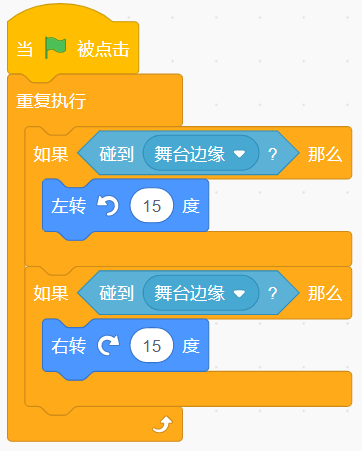
\includegraphics[width=.18\textwidth]{3a.png}
            \task 
\includegraphics[width=.16\textwidth]{3b.png}
            \task 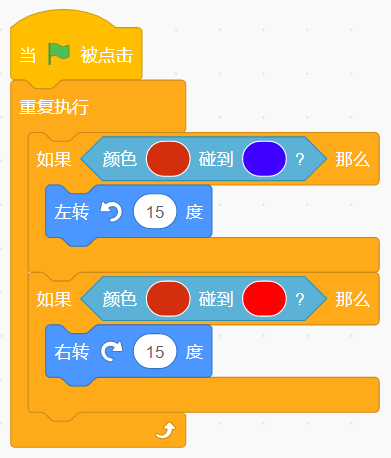
\includegraphics[width=.18\textwidth]{3c.png}
            \task 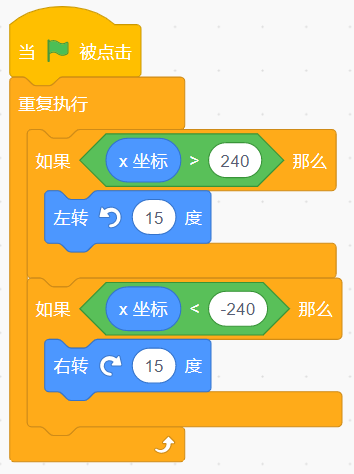
\includegraphics[width=.16\textwidth]{3d.png}
        \end{tasks}

        % 4
        \item 观察图形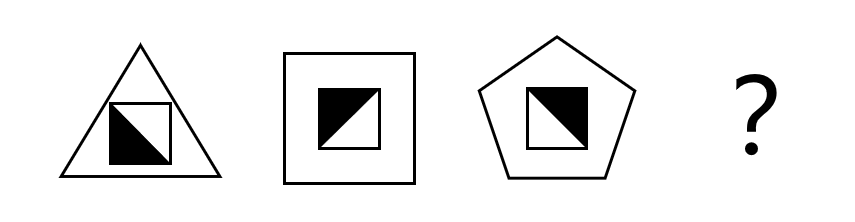
\includegraphics[width=.2\textwidth]{4.png}变换规律,问号处的图形应该是?(\qquad)
        \begin{tasks}(4)
            \task 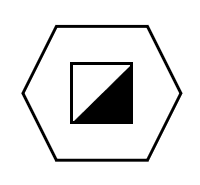
\includegraphics[width=.08\textwidth]{4a.png}
            \task 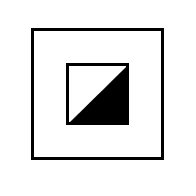
\includegraphics[width=.08\textwidth]{4b.png}
            \task 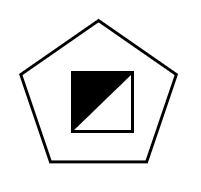
\includegraphics[width=.08\textwidth]{4c.png}
            \task 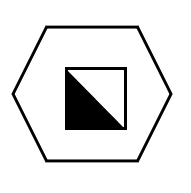
\includegraphics[width=.08\textwidth]{4d.png}
        \end{tasks}

        % 5
        \item 女孩程序和位置如下图所示,点击一次女孩后等待程序执行完毕,再点击一次女孩,说法正确的是??(\qquad)
        \begin{tasks}
            \task 第二次点击女孩,女孩说“我的宠物不是鸭子”
            \task 第二次点击女孩,女孩从鸭子处移动到Dog1的位置
            \task 第二次点击女孩,女孩说“找到我的宠物了!”
            \task 第一次点击女孩,女孩移到鸭子的位置
        \end{tasks}

        \newpage
        % 6
        \item 角色列表区如下图所示,舞台上角色显示正确的是?(\qquad)
        \begin{tasks}(4)
            \task 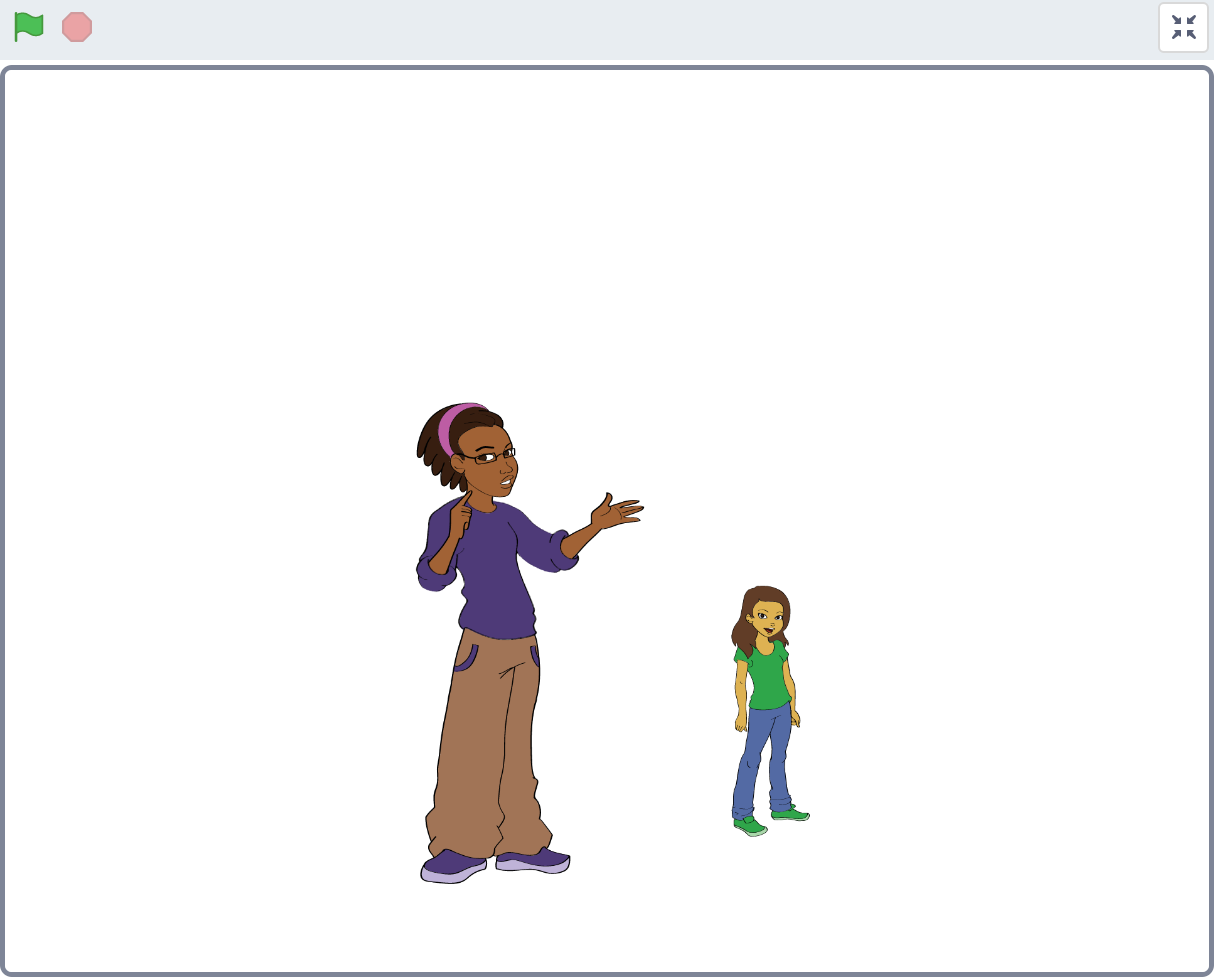
\includegraphics[width=.12\textwidth]{6a.png}
            \task 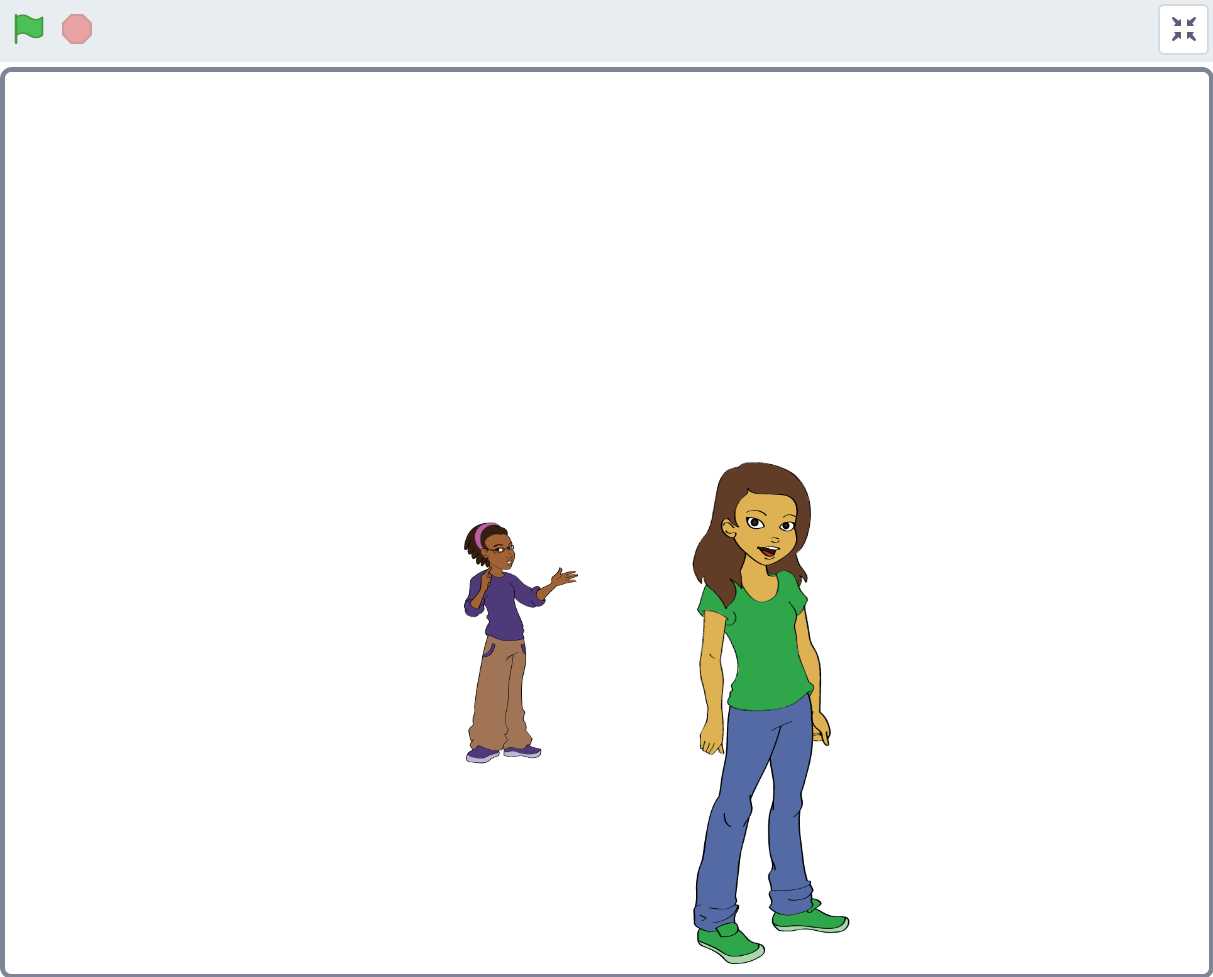
\includegraphics[width=.12\textwidth]{6b.png}
            \task 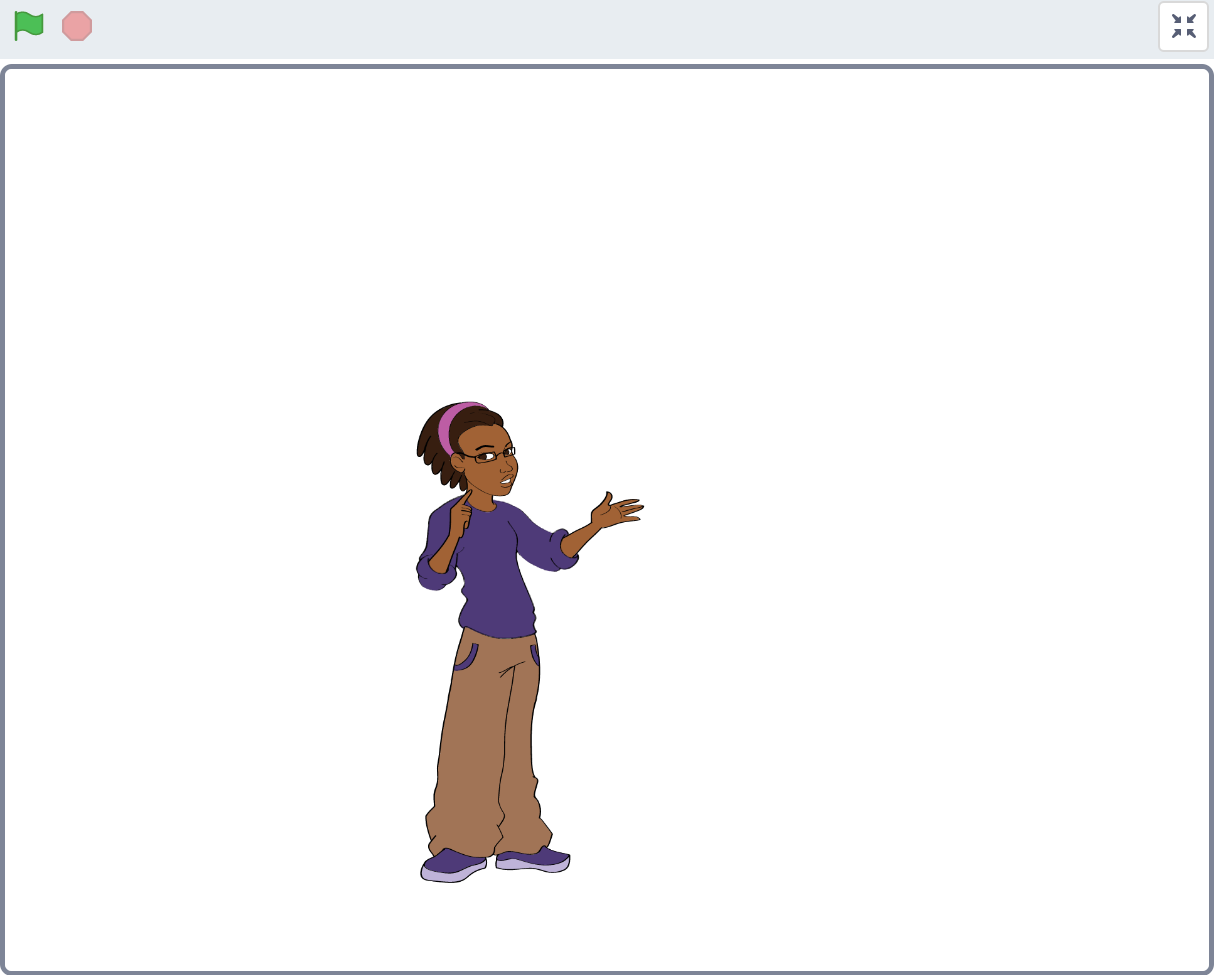
\includegraphics[width=.12\textwidth]{6c.png}
            \task 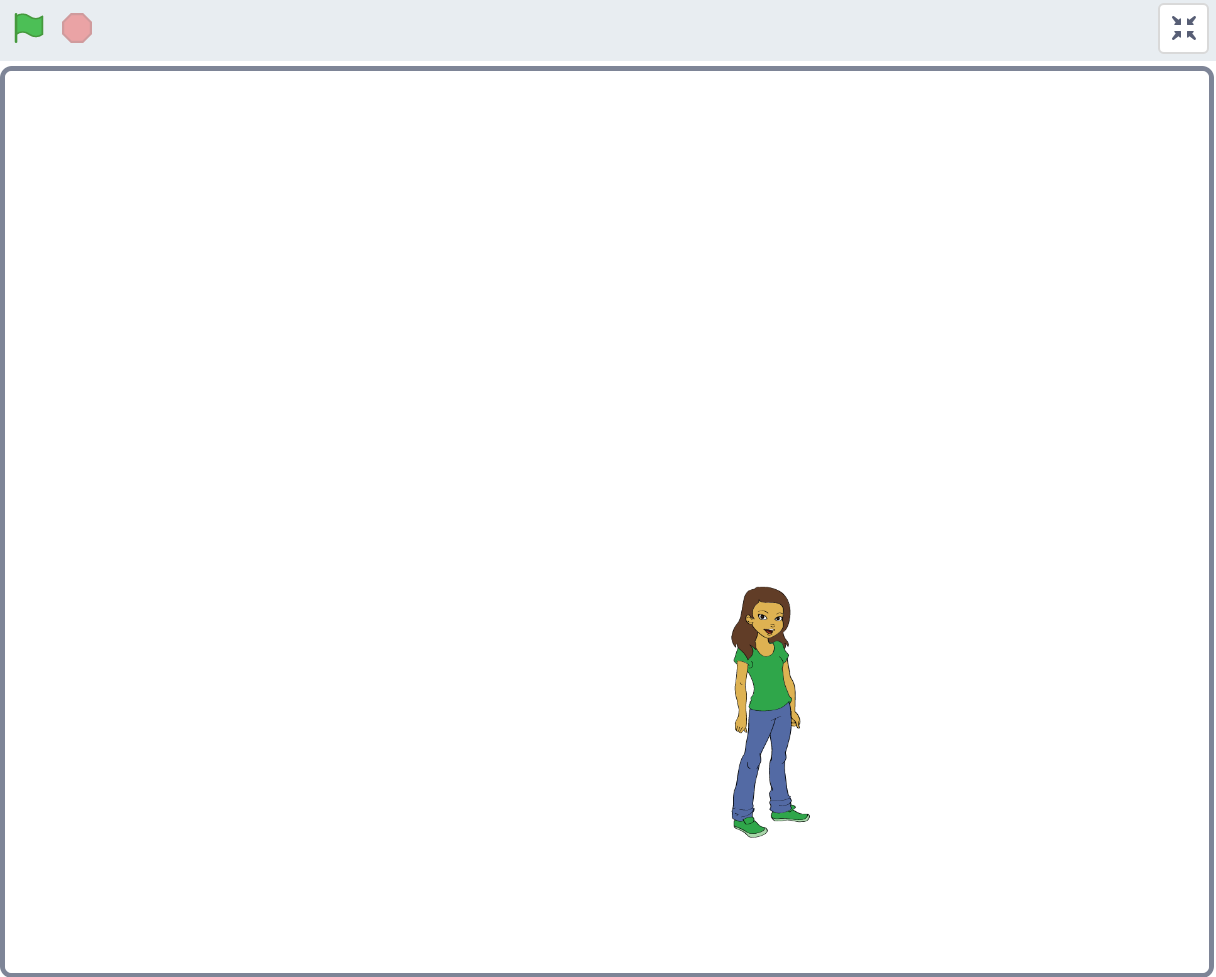
\includegraphics[width=.12\textwidth]{6d.png}
        \end{tasks}

        % 7
        \item 舞台上,气球角色挡住了小猫角色,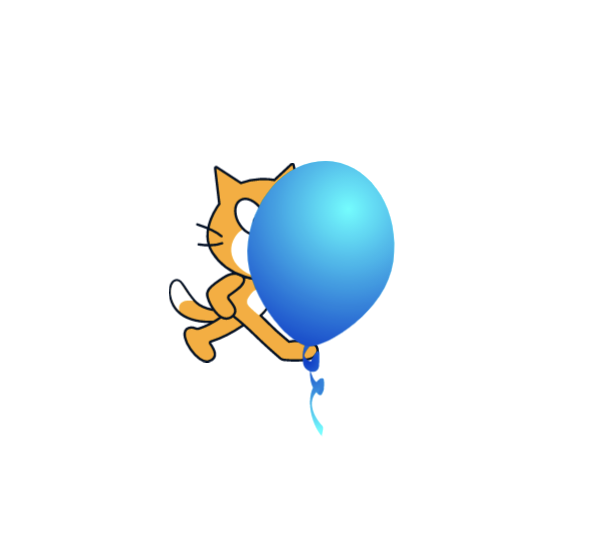
\includegraphics[width=.1\textwidth]{7.png}要想把气球放在小猫角色的后面,小猫角色执行下面哪个积木可以实现?(\qquad)
        \begin{tasks}(4)
            \task 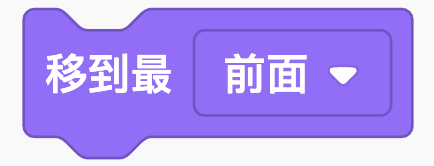
\includegraphics[width=.12\textwidth]{7a.png}
            \task 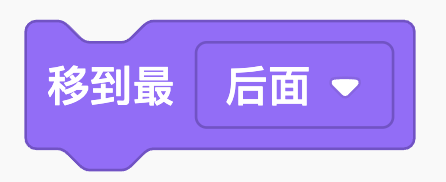
\includegraphics[width=.12\textwidth]{7b.png}
            \task 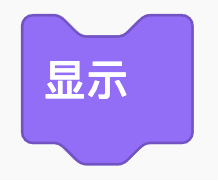
\includegraphics[width=.06\textwidth]{7c.png}
            \task 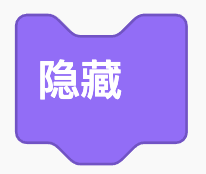
\includegraphics[width=.06\textwidth]{7d.png}
        \end{tasks}

        % 8
        \item 执行下面程序,角色会在舞台区画出什么图案?(\qquad)
        \begin{tasks}(4)
            \task 边长为 120 的三角形
            \task 边长为 120 的正方形
            \task 边长为 80  的三角形
            \task 边长为 80  的正方形
        \end{tasks}

        % 9
        \item 默认小猫角色,执行下面程序后,舞台上可以看到几只小猫?(\qquad)
        \begin{tasks}(4)
            \task 0
            \task 2
            \task 3
            \task 4
        \end{tasks}

          % 8,10,11,12 图片
          \begin{figure}[htbp]
            \centering
            \begin{minipage}[t]{.6\textwidth}
                \centering
                \begin{minipage}[t]{.48\textwidth}
                    \centering
                    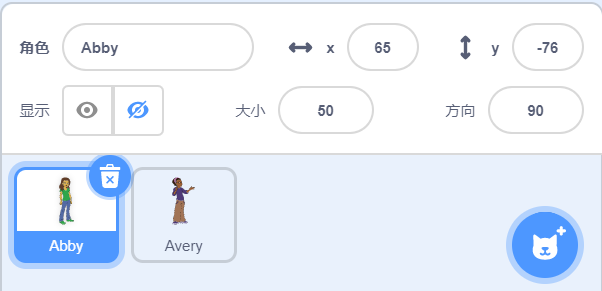
\includegraphics[width=\textwidth]{6-1.png}
                \end{minipage}
                \begin{minipage}[t]{.48\textwidth}
                    \centering
                    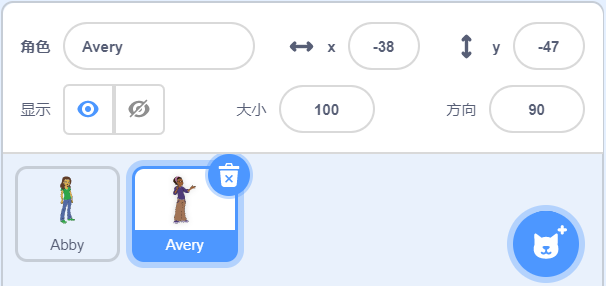
\includegraphics[width=\textwidth]{6-2.png}
                \end{minipage}
                \caption*{第 6 题}
            \end{minipage}
            \begin{minipage}[t]{.15\textwidth}
                \centering
                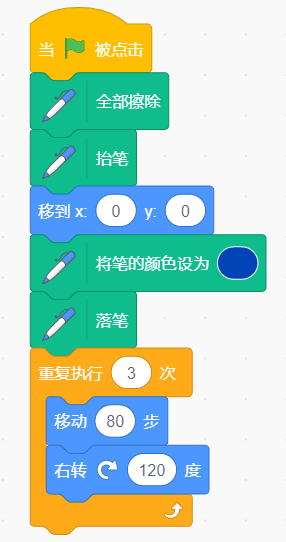
\includegraphics[width=\textwidth]{8.png}
                \caption*{第 8 题}
            \end{minipage}
            \begin{minipage}[t]{.13\textwidth}
                \centering
                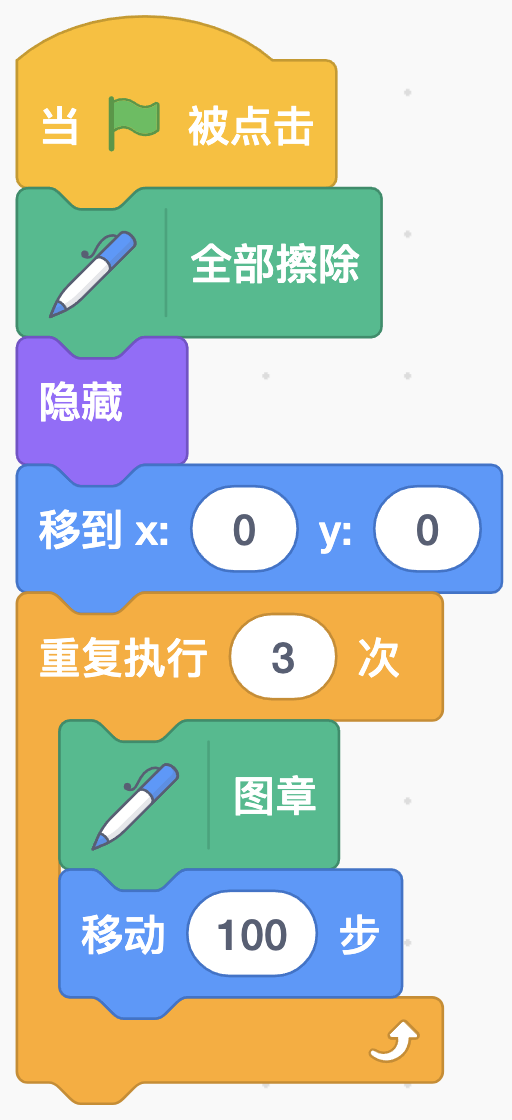
\includegraphics[width=\textwidth]{9.png}
                \caption*{第 9 题}
            \end{minipage}
        \end{figure}

        % 10
        \item 下面哪个选项,可以实现按下键盘上的右键,角色向右移动?(\qquad)
        \begin{tasks}(4)
            \task 
\includegraphics[width=.15\textwidth]{10a.png}
            \task 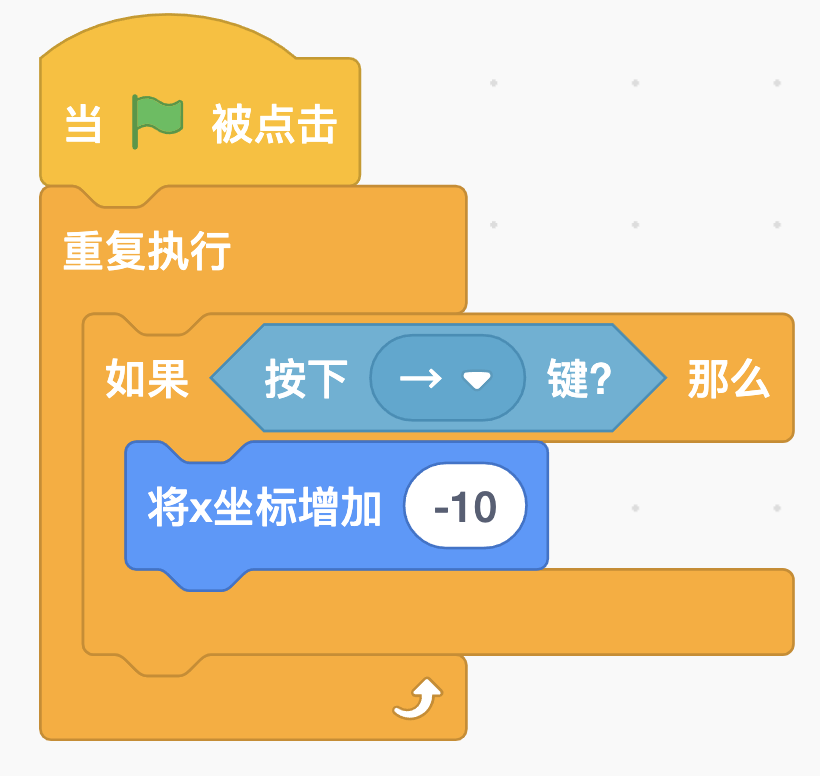
\includegraphics[width=.15\textwidth]{10b.png}
            \task 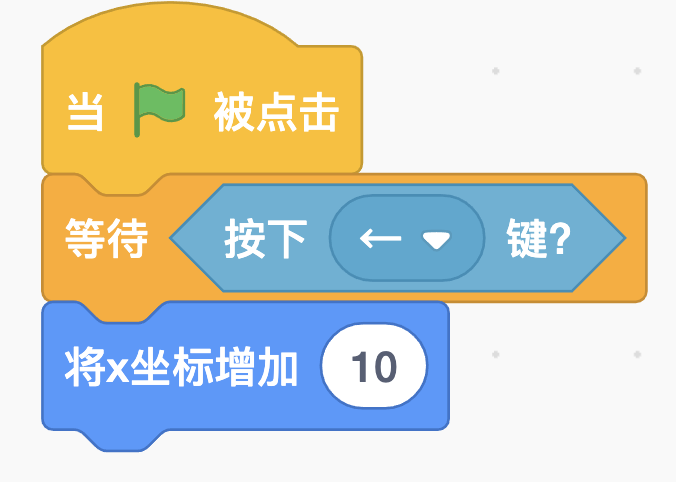
\includegraphics[width=.18\textwidth]{10c.png}
            \task 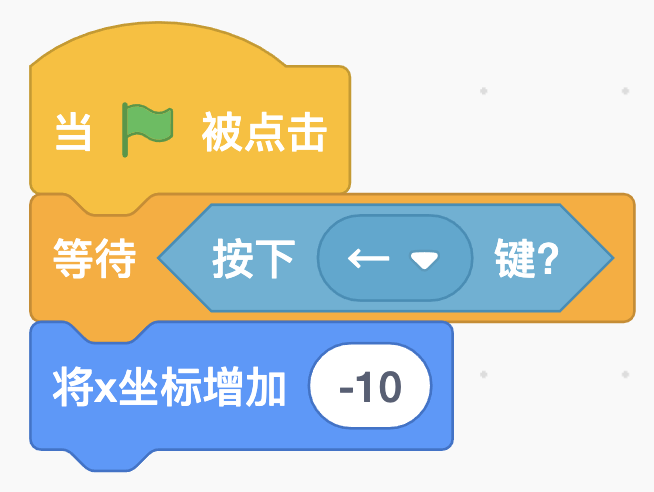
\includegraphics[width=.18\textwidth]{10d.png}
        \end{tasks}

        % 11
        \item 对下面积木描述正确的选项是?(\qquad)
        \begin{figure}[h!]
            \begin{minipage}{.3\textwidth}
                \centering
                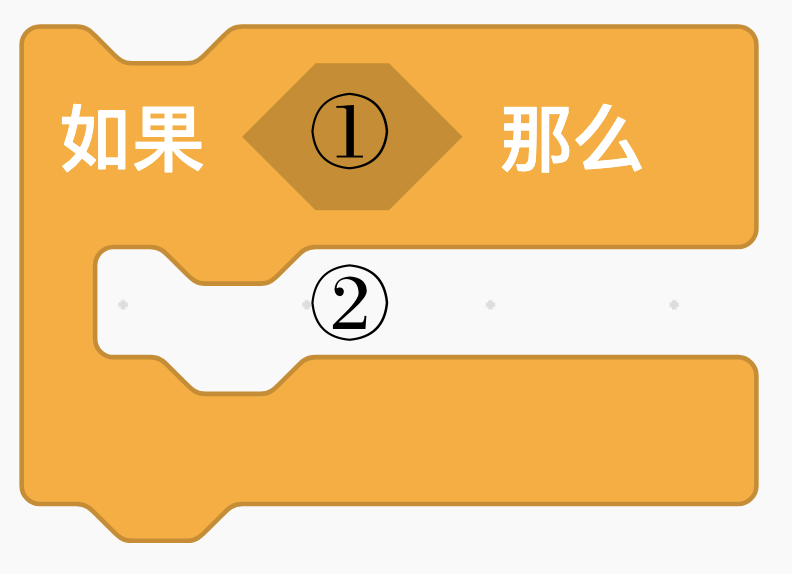
\includegraphics[width=.6\textwidth]{11.png}
            \end{minipage}
            \begin{minipage}{.6\textwidth}
                \begin{tasks}
                    \task 如果 \ding{172} 处条件为真,重复执行 \ding{173} 处的指令
                    \task 如果 \ding{172} 处条件为假,执行 \ding{173} 处的指令
                    \task 如果 \ding{172} 处条件为真,执行 \ding{173} 处的指令
                    \task 如果 \ding{172} 处条件为假,重复执行 \ding{173} 处的指令
                \end{tasks}
            \end{minipage}
        \end{figure}

        % 12
        \item 点击绿旗执行下面程序,下面选项描述正确的是?(\qquad)
        \begin{tasks}
            \task 按下空格后,角色一直移动,直到移动到舞台中心后停止移动
            \task 角色一直移动,当按下空格键后,角色移动到舞台中心后停止移动。
            \task 角色一直移动,当按下空格键后,角色立即停止移动
            \task 角色移动到舞台中心,按下空格键后一直移动
        \end{tasks}

        % 13
        \item 角色 ben 共有 4 个造型,程序如下图所示,执行前是第一个造型,点击一次绿旗,角色的造型最终停留在?(\qquad)
        \begin{tasks}(4)
            \task ben-a
            \task ben-b
            \task ben-c
            \task ben-d
        \end{tasks}
        
        \begin{figure}[htbp]
            \centering
            \begin{minipage}[t]{.19\textwidth}
                \centering
                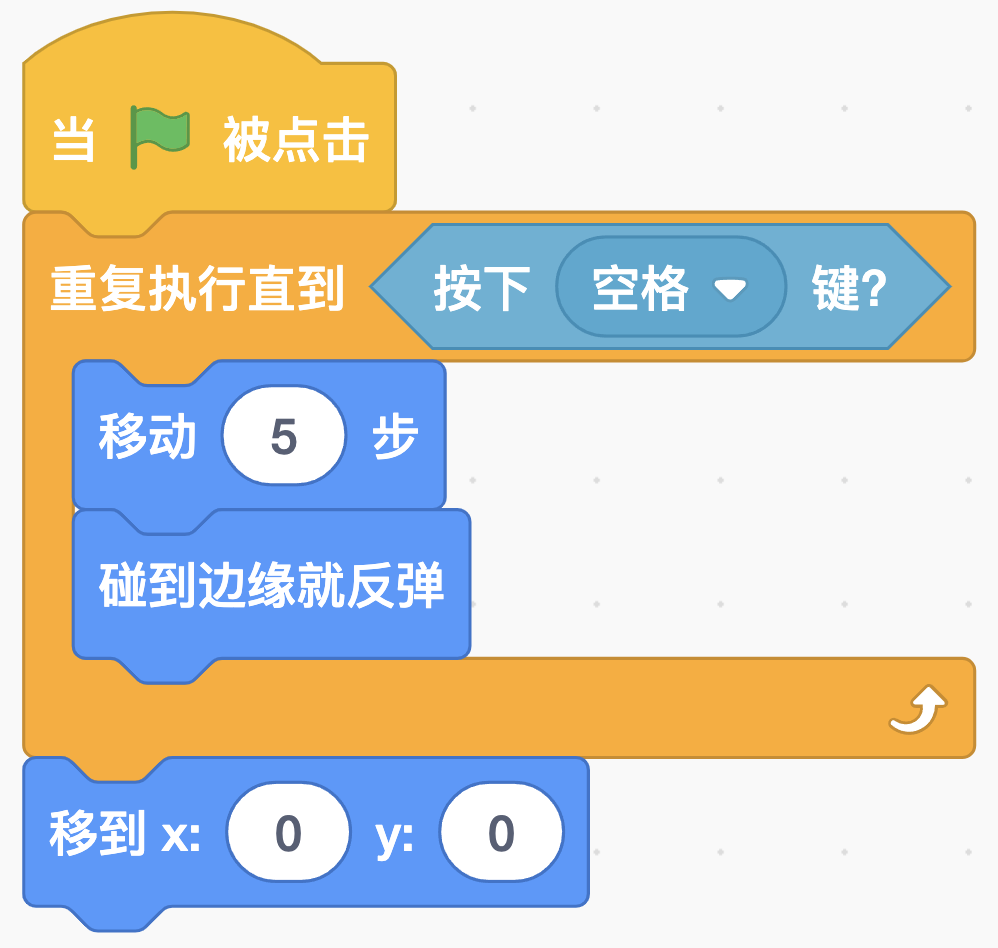
\includegraphics[width=\textwidth]{12.png}
                \caption*{第 12 题}
            \end{minipage}
            \begin{minipage}[t]{.33\textwidth}
                \centering
                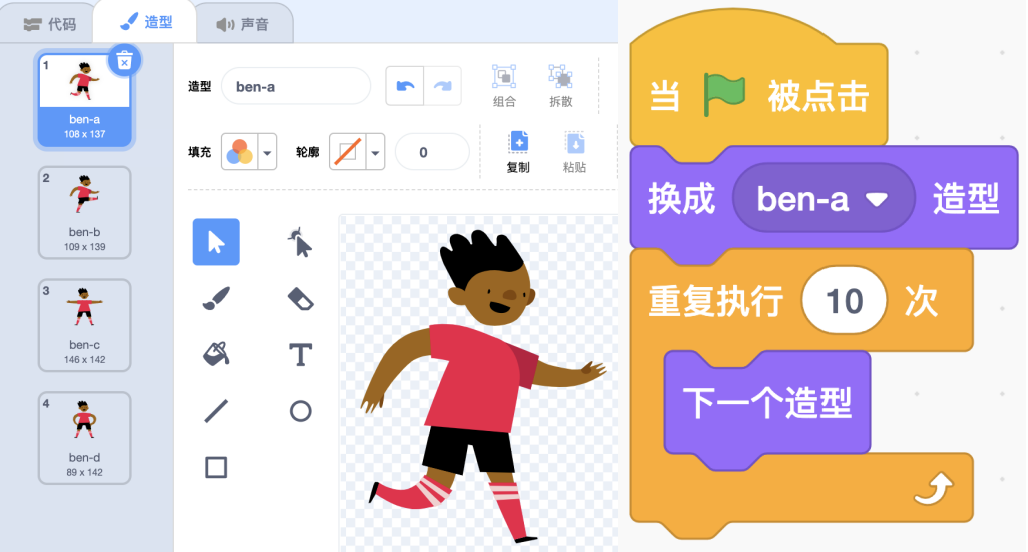
\includegraphics[width=\textwidth]{13.png}
                \caption*{第 13 题}
            \end{minipage}
            \begin{minipage}[t]{.33\textwidth}
                \begin{minipage}[t]{.33\textwidth}
                    \centering
                    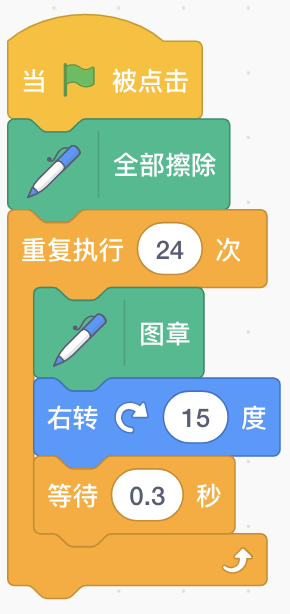
\includegraphics[width=\textwidth]{14-1.png}
                \end{minipage}
                \begin{minipage}[t]{.58\textwidth}
                    \centering
                    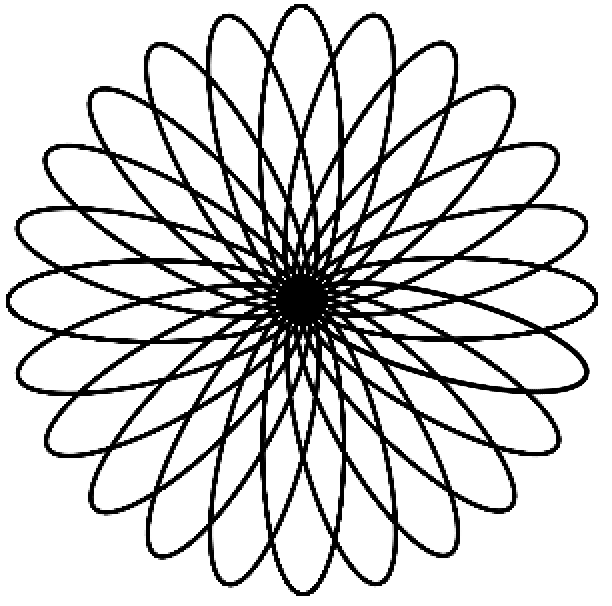
\includegraphics[width=\textwidth]{14-2.png}
                \end{minipage}
                \caption*{第 14 题}
            \end{minipage}
            \begin{minipage}[t]{.13\textwidth}
                \centering
                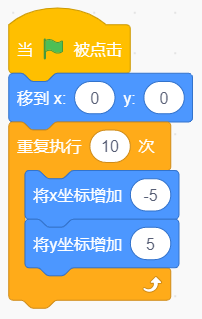
\includegraphics[width=\textwidth]{15.png}
                \caption*{第 15 题}
            \end{minipage}
        \end{figure}

        % 14
        \item 上左图的程序运行后,绘制的图案如上右图所示,下面选项中红点表示角色的中心点,中心点位置正确的选项是?(\qquad)
        \begin{tasks}(4)
            \task 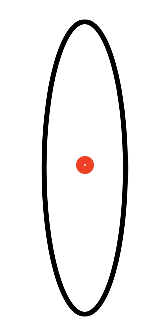
\includegraphics[width=.08\textwidth]{14a.png}
            \task 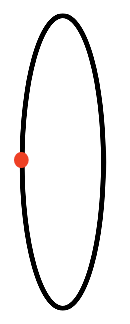
\includegraphics[width=.065\textwidth]{14b.png}
            \task 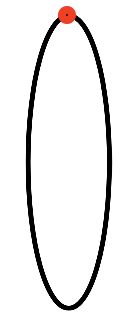
\includegraphics[width=.07\textwidth]{14c.png}
            \task 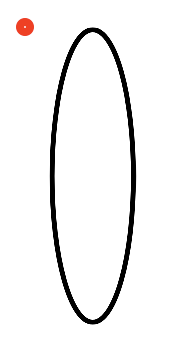
\includegraphics[width=.09\textwidth]{14d.png}
        \end{tasks}

        % 15
        \item 执行上面程序,角色的 $y$ 坐标最终为?(\qquad)
        \begin{tasks}(4)
            \task $0$
            \task $50$
            \task $-50$
            \task $100$
        \end{tasks}

        % 16
        \item 红框中填入哪个选项,可以实现:如果碰到“Bug族小兵”或者“Bug族头目”,角色说“救命!”2秒?(\qquad)
        
        \begin{minipage}{.3\textwidth}
            \centering
            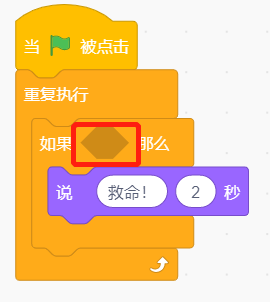
\includegraphics[width=.7\textwidth]{16.png}
        \end{minipage}
        \begin{minipage}{.64\textwidth}
            \begin{tasks}
                \task 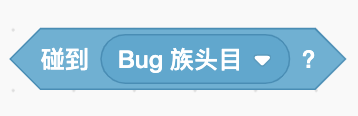
\includegraphics[width=.3\textwidth]{16a.png}
                \task 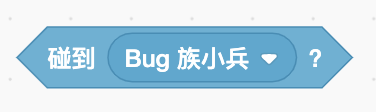
\includegraphics[width=.3\textwidth]{16b.png}
                \task 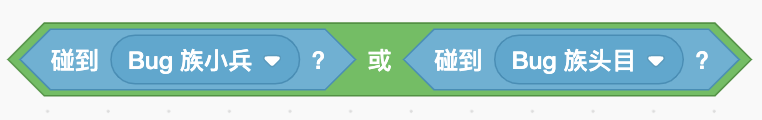
\includegraphics[width=.5\textwidth]{16c.png}
                \task 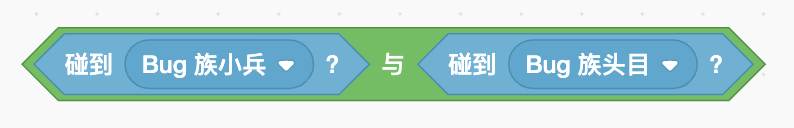
\includegraphics[width=.5\textwidth]{16d.png}
            \end{tasks}
        \end{minipage}

        \newpage
        % 17
        \item 下面两段程序可以合并成哪个选项,合并前和合并后实现的功能相同?(\qquad)
        \begin{tasks}(4)
            \task \includegraphics[width=.18\textwidth]{17a.png}
            \task \includegraphics[width=.17\textwidth]{17b.png}
            \task \includegraphics[width=.18\textwidth]{17c.png}
            \task \includegraphics[width=.18\textwidth]{17d.png}
        \end{tasks}

        \begin{figure}[htbp]
            \centering
            \begin{minipage}[t]{.35\textwidth}
                \centering
                \includegraphics[width=\textwidth]{17.png}
                \caption*{第 17 题}
            \end{minipage}
            \begin{minipage}[t]{.6\textwidth}
                \begin{minipage}[t]{.3\textwidth}
                    \centering
                    \includegraphics[width=\textwidth]{18-1.png}
                \end{minipage}
                \begin{minipage}[t]{.36\textwidth}
                    \centering
                    \includegraphics[width=\textwidth]{18-2.png}
                \end{minipage}
                \begin{minipage}[t]{.3\textwidth}
                    \centering
                    \includegraphics[width=\textwidth]{18-3.png}
                \end{minipage}
                \caption*{第 18 题}
            \end{minipage}
        \end{figure}

        % 18
        \item 上面三张图分别为舞台、笔的中心点、笔的程序,程序中的红色与舞台上的红色一致,点击绿旗,下面选项说法正确的是?(\qquad)
        \begin{tasks}(2)
            \task 鼠标点击红色,画笔的颜色会设为红色
            \task 按下鼠标,舞台区会变成红色
            \task 只要角色笔碰到红色,画笔的颜色就会设为红色
            \task 鼠标点击红色,舞台区会变成红色
        \end{tasks}

        % 19
        \item 雪人和小猫的初始位置如下左图所示,雪人面向90方向,程序如下右图所示,点击绿旗,下面选项说法错误的是?(\qquad)
        \begin{tasks}(2)
            \task 雪人到小猫的距离小于50时,说“你好!”
            \task 雪人到小猫的距离大于50时,一直移动
            \task 雪人到小猫的距离大于50时,说“你好!”
            \task 雪人到小猫的距离小于50时,不再移动
        \end{tasks}

        \begin{figure}[htbp]
            \centering
            \begin{minipage}[t]{.4\textwidth}
                \begin{minipage}[t]{.4\textwidth}
                    \centering
                    \includegraphics[width=\textwidth]{19-1.png}
                \end{minipage}
                \begin{minipage}[t]{.58\textwidth}
                    \centering
                    \includegraphics[width=\textwidth]{19-2.png}
                \end{minipage}
                \caption*{第 19 题}
            \end{minipage}
            \begin{minipage}[t]{.42\textwidth}
                \centering
                \includegraphics[width=\textwidth]{20.png}
                \caption*{第 20 题}
            \end{minipage}
        \end{figure}

        % 20
        \item 关于上面程序,说法正确的是?(\qquad)
        \begin{tasks}
            \task 角色只能同时碰到黑色、白色、红色,才会向右旋转
            \task 角色碰到黑色、白色、红色其中一种颜色,就会向右旋转
            \task 角色只能同时碰到黑色、白色、红色,才会向左旋转
            \task 角色碰到黑色、白色、红色其中一种颜色,就会向左旋转
        \end{tasks}

        \newpage
        % 21
        \item 下列选项中,与程序\includegraphics[width=.25\textwidth]{21.png}的判断结果相同的是?(\qquad)
        \begin{tasks}(2)
            \task \includegraphics[width=.18\textwidth]{21a.png}
            \task \includegraphics[width=.14\textwidth]{21b.png}
            \task \includegraphics[width=.18\textwidth]{21c.png}
            \task \includegraphics[width=.3\textwidth]{21d.png}
        \end{tasks}

        % 22
        \item 如图\includegraphics[width=.15\textwidth]{22.png}所示,当绿旗点击时,角色会说出什么内容?(\qquad)
        \begin{tasks}(4)
            \task 1
            \task 2
            \task 3
            \task 12
        \end{tasks}

        % 23
        \item 角色的坐标为$(-100, 90)$,初始方向为90,当执行\includegraphics[width=.15\textwidth]{23.png}积木后,角色的坐标变为多少?(\qquad)
        \begin{tasks}(4)
            \task $(-200, 90)$
            \task $(0, 90)$
            \task $(-100, -10)$
            \task $(-100, -190)$
        \end{tasks}

        % 24
        \item 执行下面程序后,最后角色的坐标是多少?(\qquad)
        \begin{tasks}(4)
            \task $(0, 10)$
            \task $(100, 100)$
            \task $(200, 100)$
            \task $(100, 200)$
        \end{tasks}

        % 25
        \item 执行下面程序,角色一共会移动多少步?(\qquad)
        \begin{tasks}(4)
            \task 10
            \task 20
            \task 30
            \task 60
        \end{tasks}
    \end{enumerate}

    \begin{figure}[htbp]
        \centering
        \begin{minipage}[t]{.15\textwidth}
            \centering
            \includegraphics[width=\textwidth]{24.png}
            \caption*{第 24 题}
        \end{minipage}
        \begin{minipage}[t]{.14\textwidth}
            \centering
            \includegraphics[width=\textwidth]{25.png}
            \caption*{第 25 题}
        \end{minipage}
        \begin{minipage}[t]{.29\textwidth}
            \begin{minipage}[t]{.45\textwidth}
                \centering
                \includegraphics[width=\textwidth]{26-1.png}
            \end{minipage}
            \begin{minipage}[t]{.53\textwidth}
                \centering
                \includegraphics[width=\textwidth]{26-2.png}
            \end{minipage}
            \caption*{第 26 题}
        \end{minipage}
        \begin{minipage}[t]{.23\textwidth}
            \centering
            \includegraphics[width=\textwidth]{27.png}
            \caption*{第 27 题}
        \end{minipage}
    \end{figure}

    % 判断题
    {\noindent\textbf{第二部分、判断题(共 10 题,每题 2 分,共20分.)}}
    \begin{enumerate}
        \setcounter{enumi}{25}
        % 26
        \item 如上图所示,左边流程图可以用右边积木来实现. (\qquad)

        % 27
        \item 如上图所示,点击绿旗后,按下十次空格键,小猫的 $y$ 坐标变为100. (\qquad)

        % 28
        \item 执行\includegraphics[width=.2\textwidth]{28.png}积木,角色会消失. (\qquad)

        \newpage
        % 29
        \item 点击屏幕左下角的“添加扩展”后,再点击“画笔”,可以添加画笔的所有积木. (\qquad)

        \begin{figure}[htbp]
            \centering
            \begin{minipage}[t]{.6\textwidth}
                \centering
                \begin{minipage}[t]{.4\textwidth}
                    \centering
                    \includegraphics[width=\textwidth]{29-1.png}
                \end{minipage}
                \begin{minipage}[t]{.58\textwidth}
                    \centering
                    \includegraphics[width=\textwidth]{29-2.png}
                \end{minipage}
                \caption*{第 29 题}
            \end{minipage}
            \begin{minipage}[t]{.15\textwidth}
                \centering
                \includegraphics[width=\textwidth]{30.png}
                \caption*{第 30 题}
            \end{minipage}
        \end{figure}

        % 30
        \item 执行上图程序,角色会在舞台上一直四处移动,碰到边缘反弹. (\qquad)

        % 31
        \item 下面两段程序实现的功能一样,角色碰到“怪兽”后,说“失败”2秒,整个程序结束. (\qquad)
        
        \begin{figure}[htbp]
            \centering
            \begin{minipage}[t]{.3\textwidth}
                \centering
                \includegraphics[width=\textwidth]{31.png}
                \caption*{第 31 题}
            \end{minipage}
            \begin{minipage}[t]{.3\textwidth}
                \centering
                \includegraphics[width=\textwidth]{34.png}
                \caption*{第 34 题}
            \end{minipage}
            \begin{minipage}[t]{.2\textwidth}
                \centering
                \includegraphics[width=\textwidth]{35-2.png}
                \caption*{第 35 题}
            \end{minipage}
        \end{figure}

        % 32
        \item 积木\includegraphics[width=.15\textwidth]{32.png}可以修改画笔的颜色. (\qquad)

        % 33
        \item 判断两个条件是否同时满足,可以使用这个\includegraphics[width=.15\textwidth]{33.png}积木. (\qquad)
        
        % 34
        \item 执行如上图程序,角色说“你好!”. (\qquad)

        % 35
        \item 执行如上图程序,可以画出\includegraphics[width=.2\textwidth]{35-1.png}图形. (\qquad)
    \end{enumerate}

    \newpage
    {\noindent \textbf{第三部分、编程题(共 2 题,共30分.)}}
    \begin{enumerate}
        \setcounter{enumi}{35}
        
        % 36
        \item 画正方形:
        
        1. 准备工作
        \begin{tasks}[label = (\arabic*)]
            \task 保留默认小猫角色并隐藏角色;
            \task 默认空白背景;
            \task 添加画笔模块。
        \end{tasks}
        2. 功能实现
        \begin{tasks}[label = (\arabic*)]
            \task 画笔颜色设为黑色,画笔粗细设为4;
            \task 围绕舞台中心绘制正方形,正方形的中心点坐标为 $(0, 0)$;
            \task 正方形的边长为200。
        \end{tasks}
        \begin{figure}[htbp]
            \centering
            \includegraphics[width=.3\textwidth]{36.png}
        \end{figure}

        %37
        \item 大鱼吃小鱼:
        
        1. 准备工作
        \begin{tasks}[label = (\arabic*)]
            \task 选择背景Underwater1;
            \task 删除默认小猫角色,选择角色Shark2和角色Fish。
        \end{tasks}
        2. 功能实现
        \begin{tasks}[label = (\arabic*)]
            \task 当按下“上”、“下”、“左”、“右”键时,Shark2 可以朝对应方向移动;
            \task 当按下“左”、“右” 键时,方向也跟随改变,“上”、“下”方向不变;
            \task 点击绿旗,Fish出现在随机位置;
            \task 当Shark2碰到Fish时,会张嘴闭嘴一次,这时Fish会隐藏被“吃掉”,一秒后Fish会重新在随机位置出现。
        \end{tasks}
        \begin{figure}[htbp]
            \centering
            \includegraphics[width=.3\textwidth]{37.png}
        \end{figure}
    \end{enumerate}
\end{document}